\documentclass[../main.tex]{subfiles}
\begin{document}

\chapter{Analyse} \label{Chap:Analyse}

\section{Projektets overordnede omfang}

    \begin{figure}[H]
      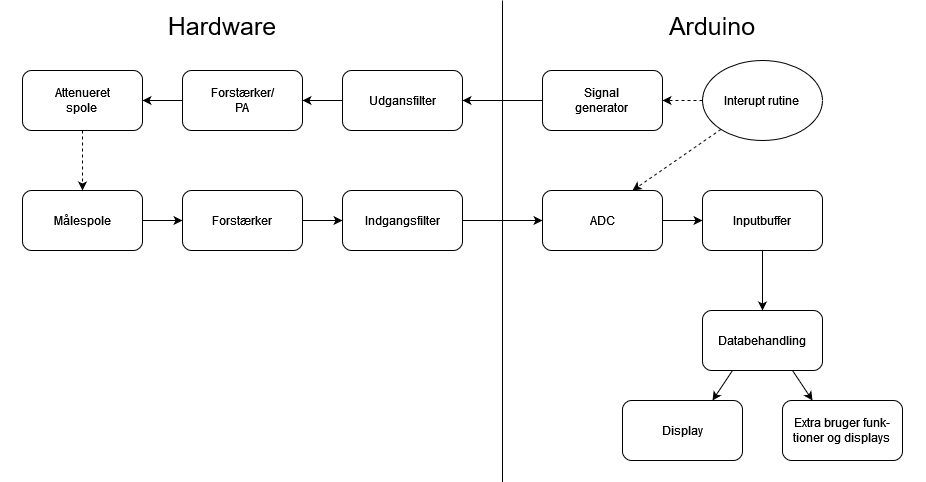
\includegraphics[width=\textwidth]{Overleaf/Pictures/Diagrammer/Overordnet projektdiagram 1.png}
     \caption{Principdiagram / blokdiagram}
     \label{fig: Principdiagram/blokdiagram}
     \end{figure}

\subsection{Hardware}
Metaldetektoren tænkes implementeret todelt med hhv. en hardware-del, bestående af diskrete komponenter, samt en mikrocontroller-del som realiseres med opsætning og kodning af en arduino.\par
Hardwaredelen tænkes implementeret i flere stadier. Først tænkes et fra arduinoen sendt signal forstærket og moduleret for at klargøre dette til at blive sendt i gennem transmitterspolen (TX).
En modtagerspole (RX) vil opfange et retursignal (RX-signal) med information omkring tilstedeværelsen af metal i metaldetektorens søgeområde, samt dennes egenskaber/type.
RX-signalet vil herefter blive forstærket og filtreret så et så vidt muligt støjfrit signal, tilpasset arduinoens måleevner, gøres klar til sampling af arduinoens ADC-modul.
\newpage
\subsection{Arduino}
Arduinoen tænkes implementeret til at skabe den oprindelige form af TX-signalet, at måle og digitalisere RX-signalet og udfører databehandling på, samt displaye, det målte RX-signal.
En tilstandsmaskine ønskes at anvendes til kontrol og styring af de forskellige funktioner.

\subsubsection{I/O signaler}
Da fasedrejningen af det målte RX-signal ønskes at anvendes til at bestemme det målte metals type er det nødvendigt at synkronisere målingen af RX-signalet med udsendelsen af TX-signalet fra arduinoen. Dette ønsker vi at implementere ved at styre udgangsfunktionsgeneratordelen og ADC'ens start-trigger gennem den samme timer, og herunder samme service rutine (ISR).

\subsubsection{Databehandling og display}
Den målte data ønskes behandlet med en variation af DFT (diskret-tids fourier transformation) for at finde signalets amplitude og fasedrejning. Ud fra dette ønskes at kunne fremvise disse værdier, samt eventuelle konklusioner baseret på data, som f.eks. det målte metals type/egenskaber.

\end{document}